\documentclass[tikz,border=10pt]{standalone}
\usepackage{amsmath}

\begin{document}
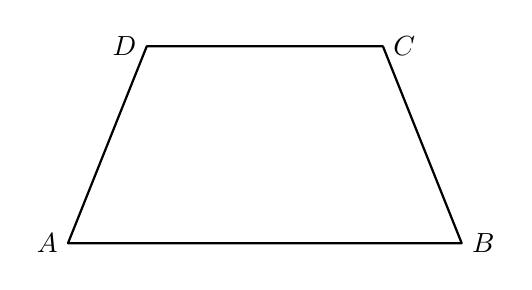
\begin{tikzpicture}[
    >=stealth, 
    thick, 
    line join=round, 
    line cap=round,
    % 定义标签样式
    label style/.style={font=\itshape\small}
]

    % --- 1. 定义坐标点 ---
    % 设置底边宽度为 5，顶边宽度为 3，高度为 2.5
    \coordinate (A) at (0,0);
    \coordinate (B) at (5,0);
    \coordinate (C) at (4,2.5);
    \coordinate (D) at (1,2.5);

    % --- 2. 绘制梯形主体 ---
    \draw (A) -- (B) -- (C) -- (D) -- cycle;

    % --- 3. 绘制顶点标签 ---
    % 根据位置自动偏移，确保标签不与连线重合
    \node[left]  at (A) {$A$};
    \node[right] at (B) {$B$};
    \node[right] at (C) {$C$};
    \node[left]  at (D) {$D$};

    % --- 4. 可选：辅助线示例（如需显示高，请取消下方注释） ---
    % \draw[dashed, thin] (D) -- (1,0) node[below] {$H_1$};
    % \draw[dashed, thin] (C) -- (4,0) node[below] {$H_2$};

\end{tikzpicture}
\end{document}